\section{Installing R and Python}
\label{sec:installing}

%TODO Aanpassen (intro en versimpelen)
In the previous chapter, we had fun with data using online platforms.
However, if you want to enjoy all the power of computational analysis
of communication, you need to install the necessary software to write,
adapt, and run code. Nowadays you may find many online and cloud
services that provide web interfaces to run code, both in R and
Python, which can be very useful depending on your
needs.
Nevertheless, we encourage you to install R and/or Python on your own
computer.
This way, you will always have access to
the basic software and packages that we will use
throughout this book and that you will likely use in the near future
in order to apply the learned techniques in your own research.

R and Python are the most popular programming languages that data
scientists and computational scholars have adopted to conduct their
work (see \refchap{introduction}). While many develop a preference
for the one or the other language, chances are good that you
will ultimately switch back and forth between them, depending on
the specific task at hand and the project you are involved in.

For Python as well as R, you need several components to create a
comfortable work environment: an interpreter for the language itself,
a program to write your code in such as an \emph{integrated
  development environment} (IDE) or a notebook, and additional
libraries (packages) to extend the functionality of R and Python.  All
of these resources are typically available for MacOS, Windows and
Linux, but keep in mind that their implementation in each operating
system might differ (for example, in the way you install the software
or when writing the absolute or relative paths in the code).

\begin{feature}\textbf{Anaconda}. An alternative to installing 
  R, Python, and optional libraries separately and as you need them
  (which we will explain in this chapter) is to install the so called
  Anaconda distribution, one of the most used and extensive platforms
  to perform data science. Anaconda is free and open-source, and is
  conceived to run Python and R code for data analysis and machine
  learning. Installing the complete Anaconda Distribution on your
  computer\footnote{\url{https://www.anaconda.com/distribution/\#download-section}}
  provides you with everything that you need to follow the examples in
  this book and includes development environments such as Spyder,
  Jupyter, and RStudio. It also includes a large set of pre-installed
  packages often used in data science and an own package manager,
  \pkg{conda}, which will help you to install and update other
  libraries or dependencies. In short, Anaconda bundles the almost all
  important software to perform computational analysis of
  communication.  So, should you install Anaconda, or should you
  install all software separately as outlined in this chapter? It
  depends. On the pro side, you just have everything installed at once and do
  not have to worry about dependencies (e.g., Windows users ususally
  do not have a C compiler installed, but some packages may need
  it). On the con side, next to that it is huge and also installs many
  things you don not need, you essentially get a non-standard
  installation, in which programs and packages are stored in different
  locations than you (or your computer may expect).  As many computers
  actually already \emph{have} Python installed (even though you may
  not know it), you also end up in a possibly confusing situation
  where it may be unclear which version you are actually running, or
  for which version you installed a package.
\end{feature}



\subsection{Installing R}

Firstly, we will install R and its most popular IDE RStudio, and we
will learn how to install additional packages and how to run a
script. R is an object-based programming language
orientated to statistical computing that can be used for most of the
stages of computational analysis of communication.  If you are
completely new to R, but familiar with other popular
statistical packages in social sciences (such as SPSS or STATA), you
will find that you can perform in R many already-known statistical
operations. If you are not familiar with other statistical packages,
do not panic, we will guide you from the very beginning. Unlike
many traditional software that requires just one complete and initial
installation, when working with R, we will first install the raw
programming language and then we will keep on installing additional
components during all of our journey. It might sound cumbersome, but
in fact it will make your work more powerful and flexible, since you
will be able to choose the best way to interact with R and especially
you will select the packages that are suitable for your project.

Now, let's install R. You can go the official R
webpage\footnote{https://www.r-project.org}, where you will find lots
of valuable information about the environment as well as the necessary
documentation for working in R.  There are different versions of R,
since there is a global community of developers that help to improve
the software continously. You should go the CRAN mirrors and click onto
any mirror (or the one you consider more close to your place of
work). Within the mirror you can download the version you need
depending of your operating system (Figure~\ref{fig:cran}). In case
you're not familiar with terms ``CRAN'' or ``mirror'', the first
refers to the \textit{Comprehensive R Archive Network}, which is an
online repository of R packages; and the second, to the server where a
copy of any package is available for download.

\note{If you use Linux, you may want to install R via your package
  manager (such as \texttt{apt} on Debian and Ubuntu) instead.}


\begin{figure}
\centering
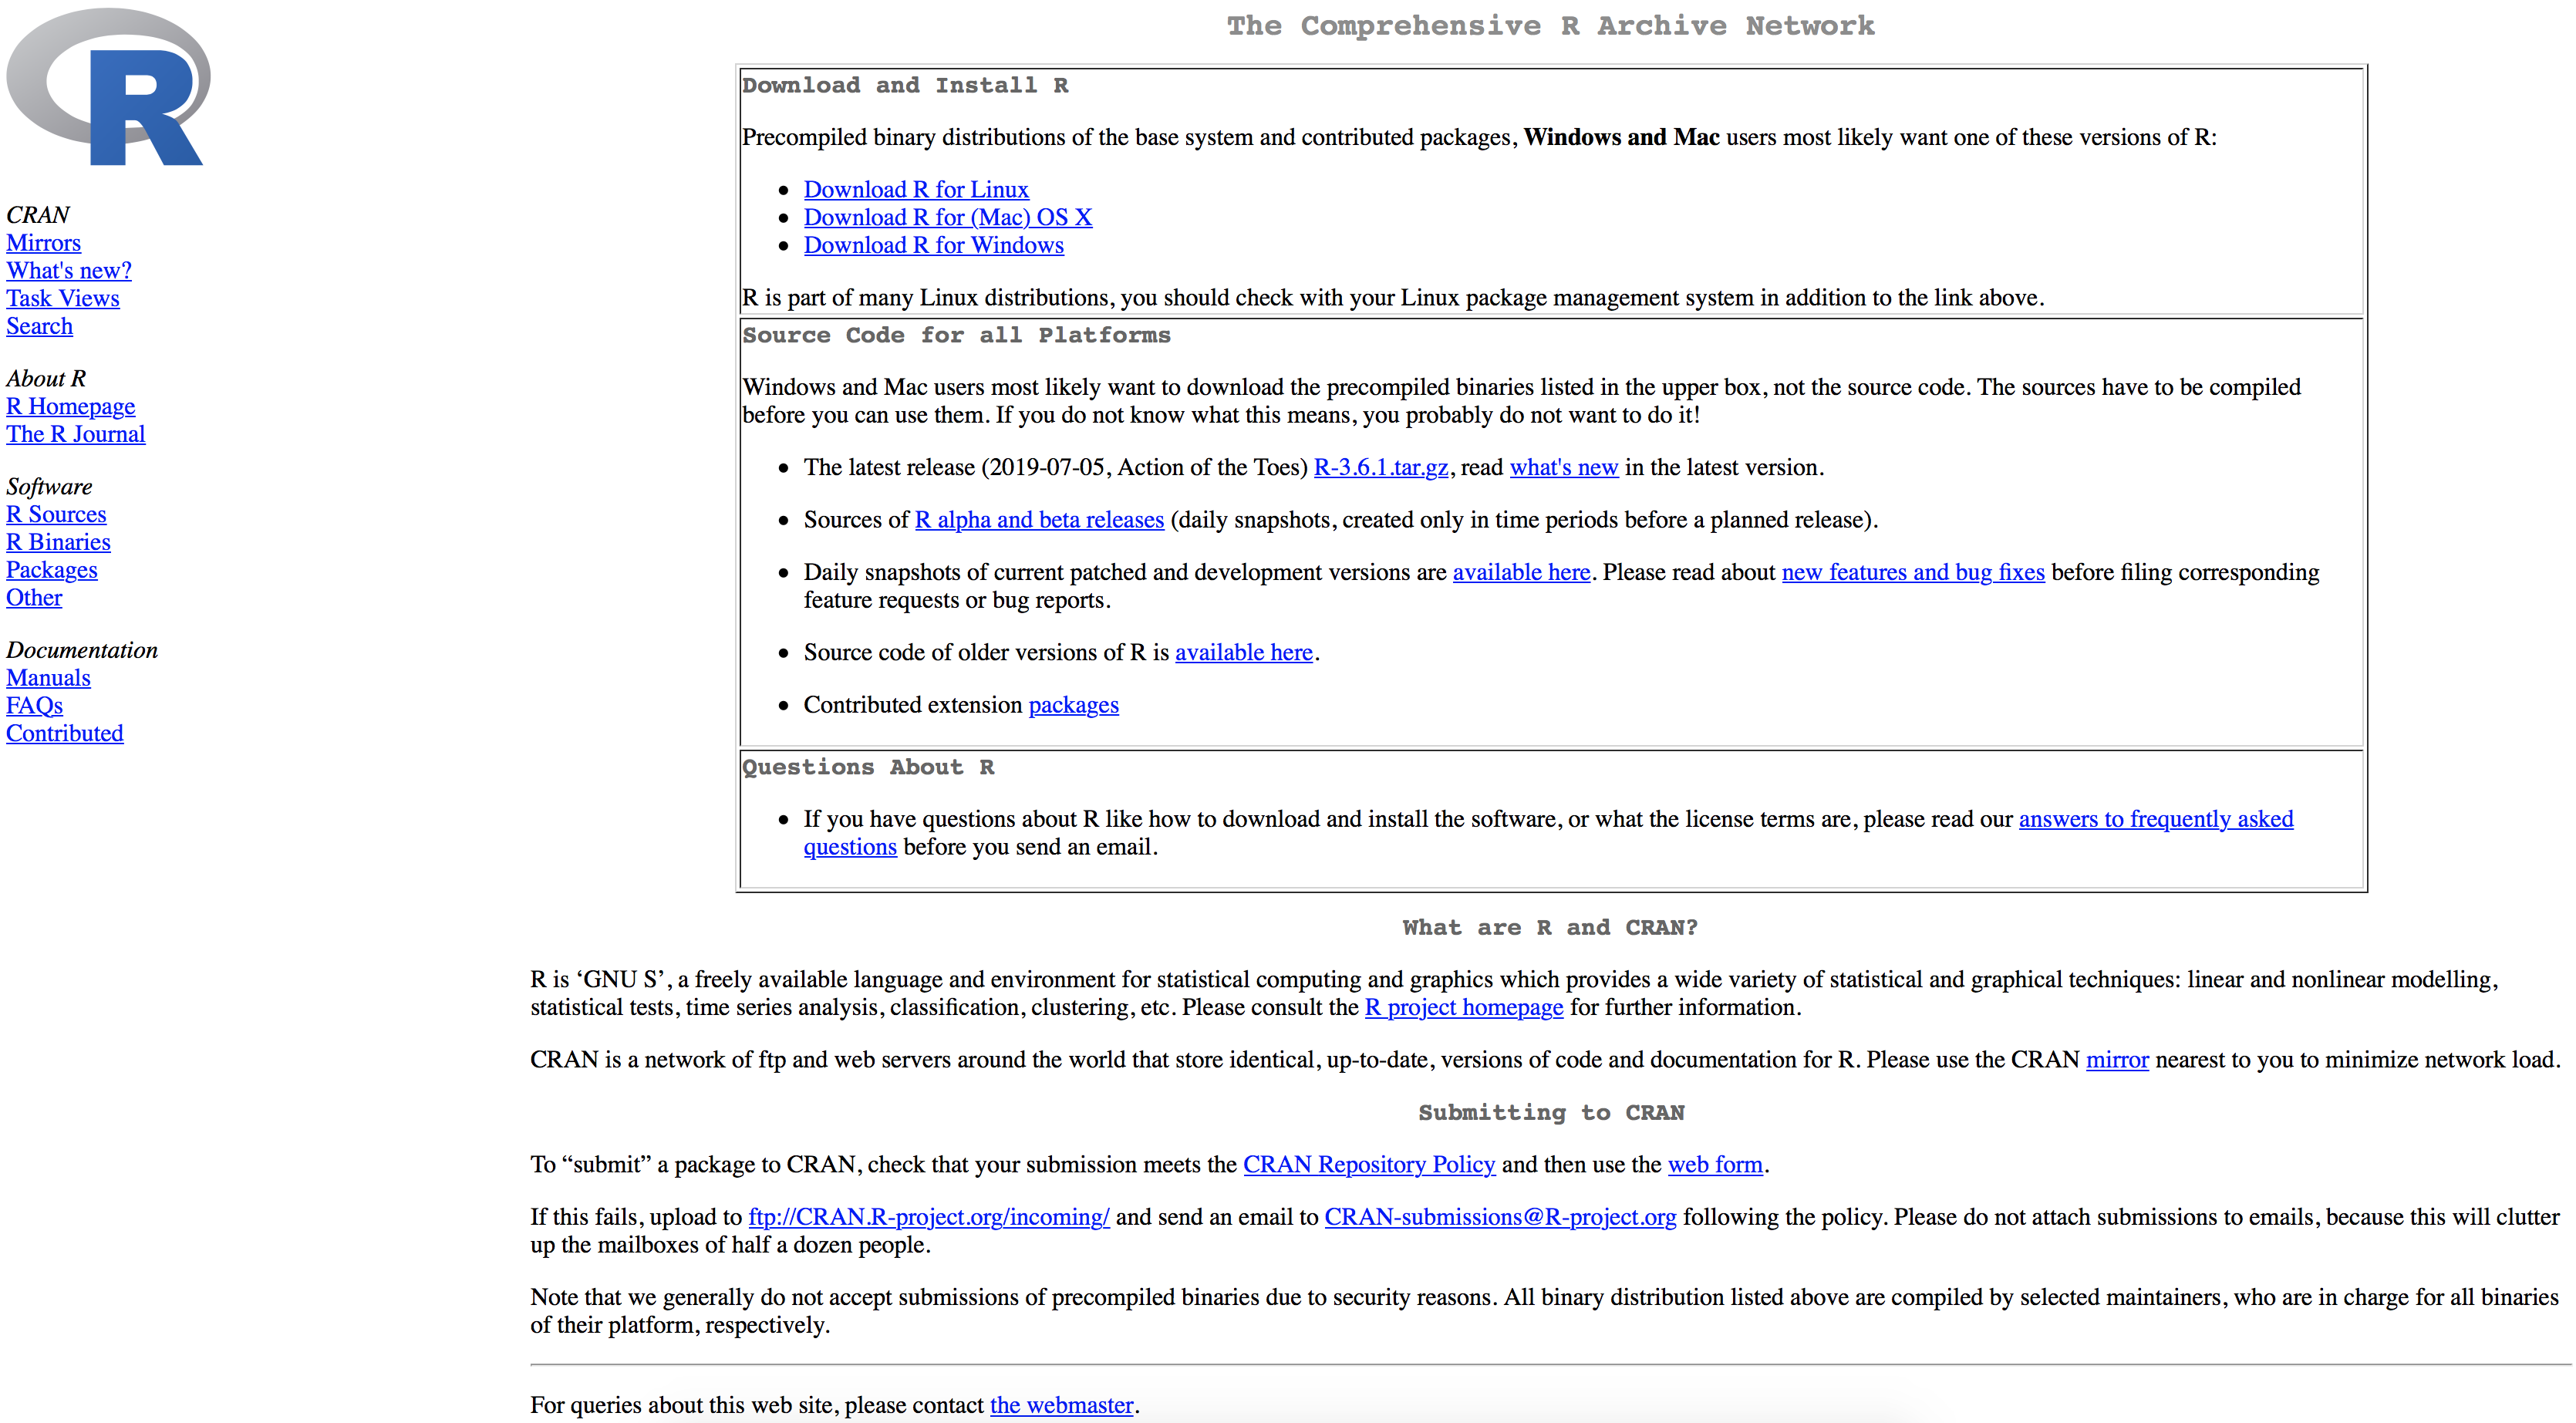
\includegraphics[width=0.9\linewidth]{figures/ch3_cran}
\caption{The Comprehensive R Archive Network.}
\label{fig:cran}
\end{figure}

Once you have downloaded and installed R on your computer (follow the
instructions on the page for each operating system), you will be able
to open an R console (Figure~\ref{fig:r_console}), where you can
perform all operations, from reading datasets to execute sophisticated
data analysis. If you are new to computer science jargon, it is worthy
to clarify what a \textit{console} is and what is the difference with
a \textit{script}. In a console, you can write and execute commands
line-by-line. In fact, all computers and operating systems have
terminals or consoles, which help us to interact with the machine,
from listing files of a given folder (e.g. command \texttt{ls} on
Linux and MacOS) to install software, apps or utilities. The point is
that any console is an active tool that normally executes the line or
group of lines after you press the \textit{enter} button.
If, instead of typing each command line-by-line into your console,
you put several of such command lines into a text document, we call it a \textit{script}.

If you want to execute some more complex set of code lines, you may
wish to write and test them in a separate file (the script) that you
can save and also run from the console. This distinction is very
useful in R, as you will normally work with both, an R script file and
an R console, in order to run your computation.

\begin{figure}
\centering
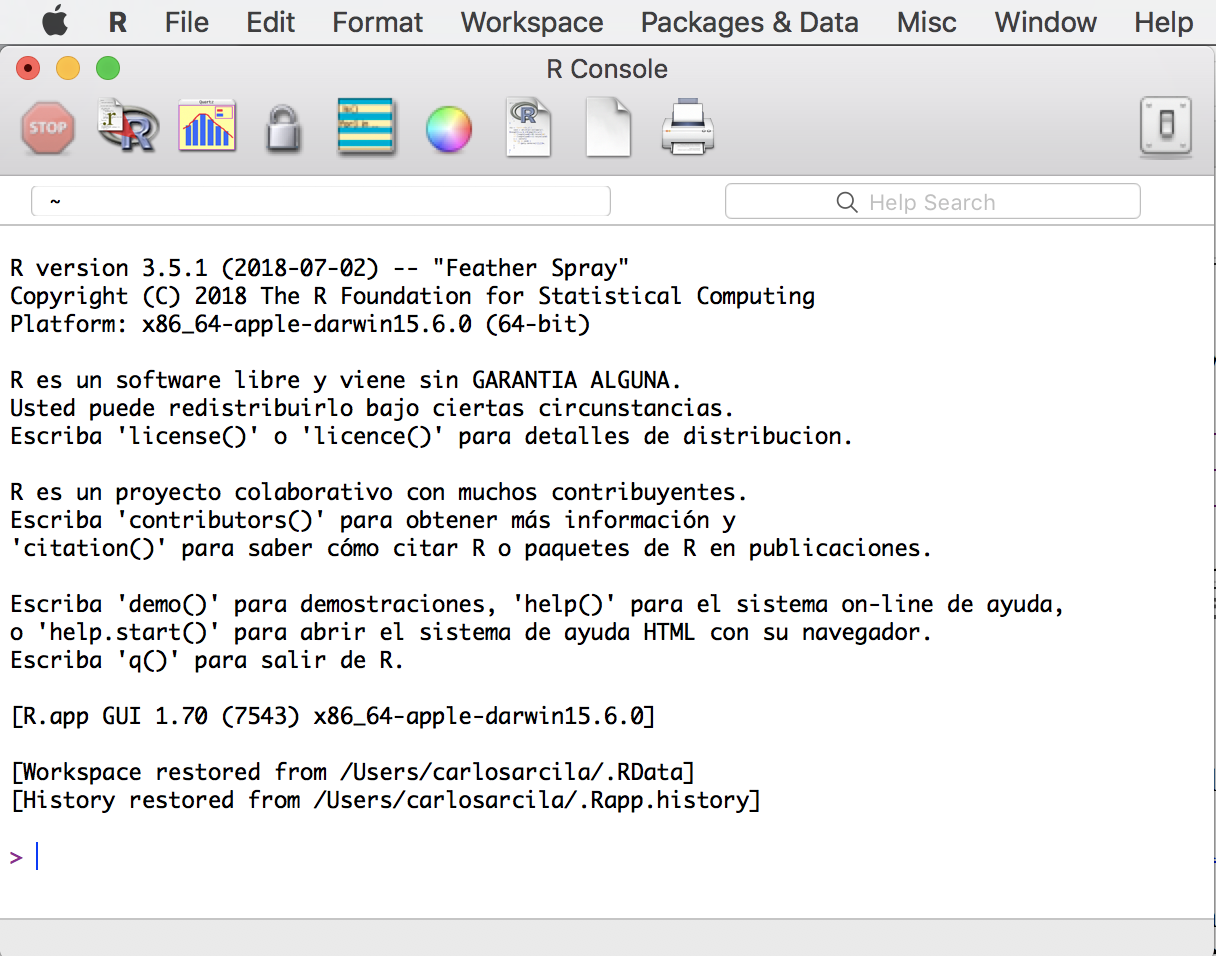
\includegraphics[width=0.9\linewidth]{figures/ch3_r_console}
\caption{R Console.}
\label{fig:r_console}
\end{figure}

\newcommand*{\icon}{
\includegraphics[scale=0.8]{figures/document_icon}}%
\newcommand*{\doc}{
\includegraphics[scale=0.7]{figures/r_document_icon}}%
\newcommand*{\rcom}{
\includegraphics[scale=0.8]{figures/r_icon}}%

In the R Console you will just have an empty line beginning with the
sign \textgreater, where you can write any command, and also a menu
with some useful icons. For example, the empty document icon \icon
\ will allow you to create a new R document and write there your
code. You can later use R document icon \doc \ to modify any given
script or the general R icon \rcom \ to run the script or to load data
in R. On the upper menu you will also find convenient tools such as
Workspace or Packages \& Data. Because R is an
object-orientated programming language, which means that all
operations are performed with objects that we create or import, from
simple variables to complex recursive functions. If you create an
object \texttt{x} with the value 17 (|x = 17|), this object will
be loaded into RAM memory so you can access by just typing \texttt{x}.
The menu Workspace will let you know which objects
have been uploaded to this virtual space. We will go back to this
issue later in this chapter when we discuss statements, expressions,
variables, functions and methods. R can perform many statistical operations with its
raw language, but one of its greatest advantages is that we can use
existing packages (also called libraries) that others have created to
simplify our coding and to expand our possibilities in data
analysis. You can find these packages in the CRAN, ensuring that there
has been a minimum set of verification steps for that code, or
directly from a developer webpage or repository. The menu Packages \&
Data will help you to manage and install packages, as well as to load
pre-existing data (freely available datasets we can work with).

If you are unfamiliar with dealing with datasets in a coding
environment, probably the first package you will be willing to install
is \pkg{R Commander}\footnote{https://cran.r-project.org/web/packages/Rcmdr/index.html},
or \pkg{Rcmdr} for short, which is a graphical user interface for R that
helps you to interact with data in a more visual way, similar to SPSS.
You can install this package either by using the R Package Installer
tool (Menu \textgreater Packages \& Data \textgreater Package
Installer), or by typing the next syntax on your R Console:

\codex{chapter03/installpackages.r}

Be patient, it will take some time to download and install on your
local computer all the files and dependencies necessary to run \pkg{R
  Commander}. The good thing is that you have run your first line of
code and you will notice that it is not that difficult; most of the
commands you will use will follow a similar logic. In this case you
have a native command (install) with a module (packages) and an
argument (``Rcmdr'') with an option (dependencies=TRUE). It is worth
mentioning that once you have installed any package on your computer,
you have to import it it in the R environment every time you are going
to work with it. This means that you have to indicate either on your R
console or R Document, which libraries you will be using, so the
program can load the package, which you can do with the command
\fn{library}. You can for instance write |library(base)| to import
the library named ``base''. Whenever you want to know more about a
command you can ask for documentation using the |?| symbol,
e.g. |?library|.

Now, let’s load R Commander by typing |require(Rcmdr)| into the R consule.

In this case, by loading \pkg{Rcmdr} a pop-up window will be displayed
with the graphical interface to work with data and run basic
statistics. In most other cases, no window will show up, but the
package will be loaded in the backend so you can use all its
functions. For example, if we are working a on an R script (.r or .R)
where we write a set of instructions that need any particular package
we should call that package in the file before it performs any
operation included in it (by just entering a line such as
|library(<the_package>)|.

With this line you ensure that you will not get an error message
warning you that certain function does not exist or has not been
properly called when your are running the script.

Now that you have learned how to install R and its packages on your
computer, we should move on to get familiar with additional resources
that are of great help when working with R. In particular we introduce
RStudio, which is an IDE (Integrated Development Environment),
free of charge and open source that will
make our computational journey with R much more friendly and
easier. Among many other advantages, in this environment you will have
a workspace where you can simultaneously visualize your R documents
(.r files), the R console, the objects or variables you load to memory
and files or packages you are dealing with. You can find a desktop
application that will run locally on your computer (RStudio Desktop)
or a web-server version that you can install on a remote server and
run from any web browser via Internet (RStudio Server). If it is your
first time on this environment, we encourage you to download and
install RStudio Desktop (figure~\ref{fig:r_studio}) from its official
website\footnote{https://www.rstudio.com/products/rstudio/download/}. As
in the case of R, choose the appropriate installation file for
your operating system (MacOS, Windows, Linux) and get the latest
version.

\begin{figure}
\centering
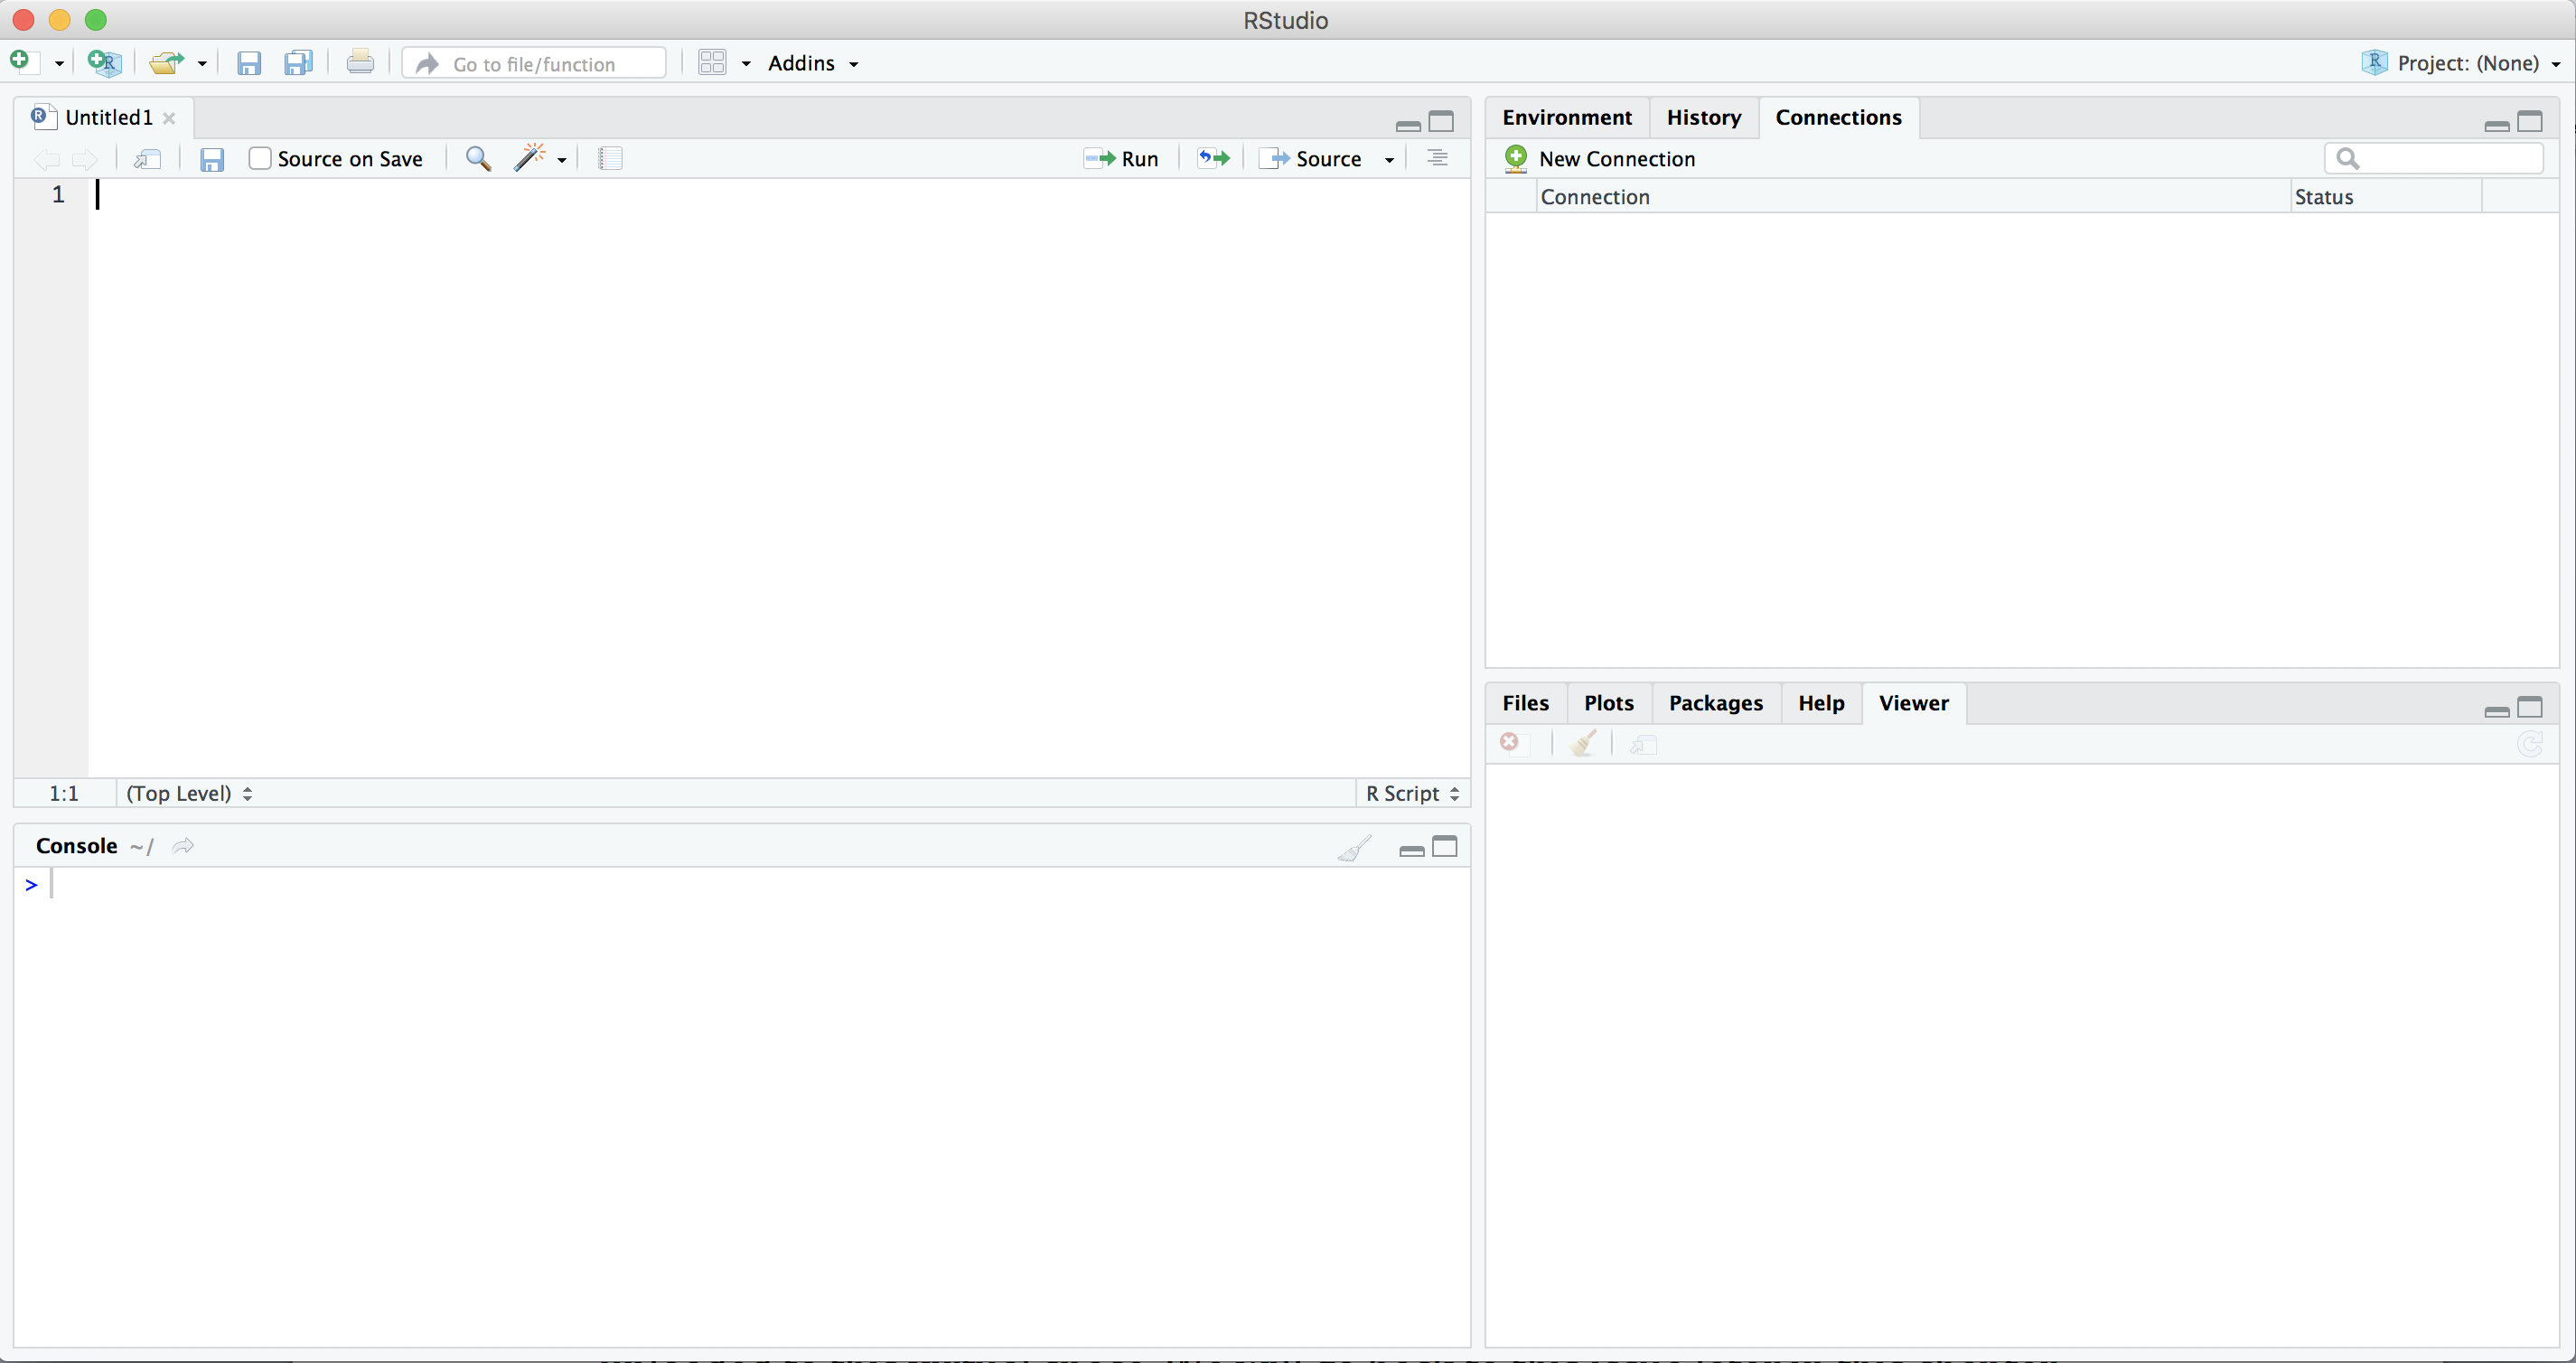
\includegraphics[width=0.9\linewidth]{figures/ch3_r_studio}
\caption{RStudio Desktop}
\label{fig:r_studio}
\end{figure}

In RStudio you will see by default four main integrated windows (you
may later reconfigure it), and the upper menu. In the up-left window,
you can visualize and edit all the files you will work with, in
special R documents (|.r|), data, and R Markdown documents (|.rmd|).
If it is the first time you hear about Markdown, keep this format in
mind because it is a markup language for plain text that will help you
to work with reproducible R documents based on a very simple syntax
and ready-to-export to most universal formats such as HTML or PDF. The
down-left window is the R console where you can directly write a
syntax or where your will get the outcome from the code you have
written and run in the R document. Look at the up-left window
and notice that there is a button named \emph{run}, which you will
often use. By selecting partial or total lines of code in your script
and clicking on this button you will execute the code and get the
results in the console.  As you will realize with the first practices,
it will be very useful to have the script in one window and gradually
run parts of the code, instead of executing the whole document at once
or to run it line by line in the console.

On the right side of RStudio workspace you will find two additional
windows. In the up-right window there are two or more tabs:
\emph{environment} and \emph{history}, and depending on additional
packages you may have installed maybe some more.  In
\emph{environment} you can manage your workspace (the set of elements
you need to deploy for data analysis) and have a list of the objects
you have uploaded to it. You may also import datasets with this tool.
It is also possible to save your ``workspace'' or open a previous one.
However, relying on this functionality is often not a good idea: it
will only save the state of your current session, whereas you most
likely want to save your R syntax file and/or your data instead.
If you have your raw input data (e.g., as a csv file, see \refchap{filetodata})
and a |.R| syntax file (by clicking on File/Save As), you can always
reproduce what you have been doing. If you only have a snapshot of
your workspace, you know state in which you arrived, but cannot
necessarily reproduce (or change) how you got there. A better idea
to bundle everything that you need (data and code) is to create (and
later re-open) a new project (via File/New Project), which will
initialize a new folder to work in. Saving your workspace, in contrast,
is usually not necessary, even though RStudio may ask you for it.

In \emph{history} you will
have an inventory of code executions, which you can save to a file, or
move directly to console or to an R document. In the down-right window
you will have five more useful tabs. In \emph{files} you can explore
your computer and manage all the files you may use for the project,
including importing datasets. In \emph{plots}, \emph{help} and
\emph{viewer}, you can visualize the outputs figures, documentation
and general outcomes, respectively, that you have executed in your
script. Finally, the tab for \emph{packages} will be of great
utility since it will let you install or update packages from CRAN or
even from a file saved on your computer with a friendly interface.


\subsection{Installing Python}

Now that you have installed R and RStudio, let's change to Python. As
many computational scientists do, we will jump from one application to
another throughout this book, so do not worry if you have to wear two
hats the same day, even at the very same time! The first thing will be
to install Python on your local computer (though some operating
systems come already with it as a default). As explained in \refchap{introduction}, Python is an object-orientated programming language
and it is probably the favourite language of computational and data
scientists in all disciplines around the world. There are different
releases of Python, but you will usually find a distinction between
versions of Python 2 and those of Python 3, since some syntax and
functions change from one to another. In this book, we will explain
Python 3.x and all our examples and exercises will be written for this
version. Notice that you might install different versions of Python on
your local computer, and also create specific virtual environments
(including a Python version and all its libraries and dependencies).
By doing this, you will be able to run any version depending on your
needs. Thus, if you do not have already Python on your
computer \footnote{There are different ways to check if you already
  have it. For example, if you are in MacOS, you can open your system
  terminal and type \texttt{python -V} or \texttt{python --version}, and
  you will get a message with the version that is working by default
  in your computer or that has been set as an environment
  variable. There might be different versions already installed, so
  you might check directly for them: \texttt{python2 --version} or
  \texttt{python3 --version}.}, the first thing will be to download it
and install it from its official
webpage\footnote{https://www.python.org/downloads/}, selecting the
right software according to your operating system (Windows,
Linux/UNIX, Mac OS X).

\note{If you use Linux, you may want to install Python via your package
  manager (such as \texttt{apt} on Debian and Ubuntu) instead.}


During the installation, you will be informed that some additional
features will be installed along with Python: normally an
\emph{integrated development environment} called \pkg{IDLE}, a package
manager called \pkg{pip} and \emph{documentation}. Even though more
advanced IDEs are available (for instance, you may like \pkg{spyder},
which looks a lot like \pkg{Rstudio}, or \pkg{pycharm}, which has a lot of functionality that appeal to advanced programmers), IDLE will
provide you with a basic interface to work with Python files (|.py|)
and the Python console. \pkg{pip} is a basic package that will help
you to install and manage more software packages within Python. And
documentation will provide you with basic help to work in this
programming language.  In addition, you might be asked if you
want to add Python to your path, which means that you set the
\emph{path variable} in order to call the executable software from
your \emph{system terminal} just by typing the word |python|. We
recommend selecting this option.  If you have never worked before with
the system terminal of your computer, probably this is a good
opportunity to know what and where it is. With this terminal you can
interact with your machine and navigate through your files, create new
ones, install programs, execute scripts, etc.  Everything you already
do in your friendly and graphic interface in Windows, MacOS or Linux,
but performing it only with commands and code. Well, if you already
downloaded and installed Python, you may open your system
terminal\footnote{The terminal will look slightly different depending
  on your operating system. In MacOS or Linux you can find it the
  `Terminal' in the Utilities folder in Applications; and in Windows
  you can get the `Command Prompt' in the Accessories folder in the
  All Programs menu.}  and launch Python from it! First, type
|python --V| and press enter to check your current installed version and then
just type |python| and you will open the software from the very same
system terminal.

\begin{figure}
\centering
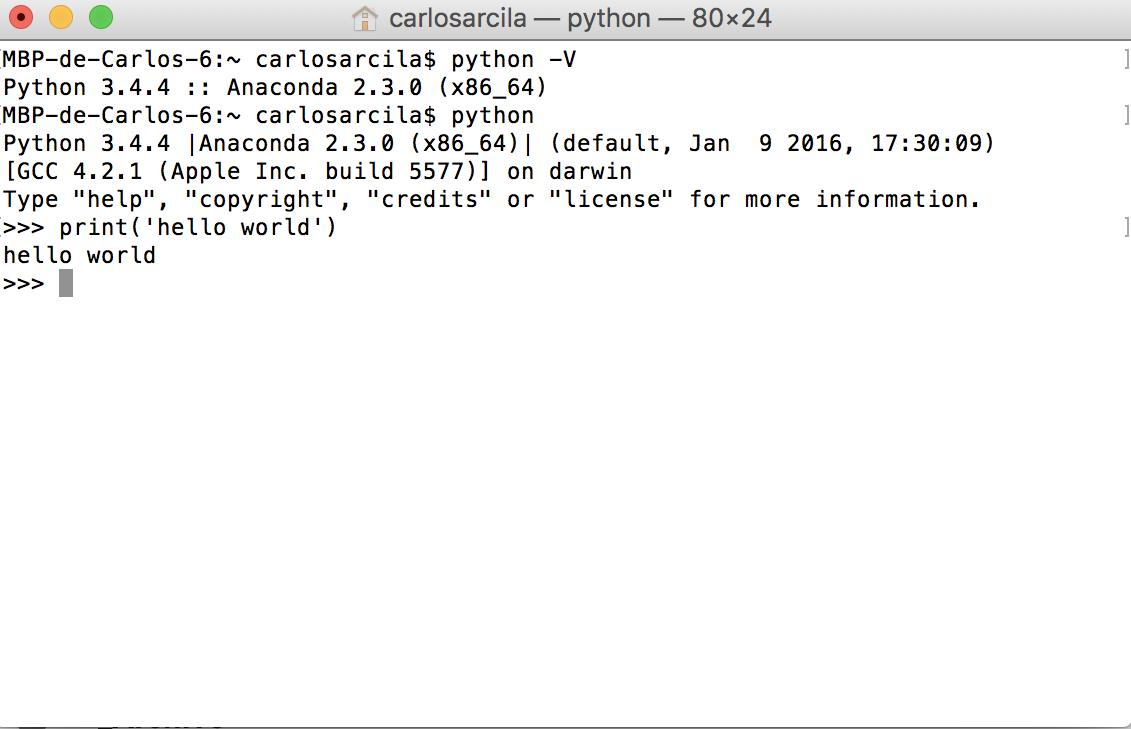
\includegraphics[width=0.9\linewidth]{figures/ch3_python_from_terminal}
\caption{Python launched from the Terminal.}
\label{fig:python_from_terminal}
\end{figure}

So, welcome to Python. You are now in the Python console, from where
you freely operate this programming language. As it is a console,
every line of code you type will be executed by pushing enter onto
your keyboard, which means that if you have complex code you will
mostly prefer to write the script in a Python file (.py) or similar
(i.e. a notebook) and then run this file. However, as a first exercise
it will be worth to keep the Python console open and write your first
line of code on it, using the native function \fn{print} (see \refex{helloworld}).

\pyrex[output=py,input=py,caption=Your first program]{chapter03/helloworld}

After running this line, you will get your first result or
output (see also Figure~\ref{fig:python_from_terminal}), which will be to
display on the screen a sequence of characters, called a
\emph{string}. You might tell your colleagues that you have written
your first computer program, just as many computer scientists have
done so in their first programming class. We will come back to coding
in Python in the next sections. Now, let’s try to install some
packages. Remember, that similar to R, in Python we can build every
function from scratch, but there are many libraries or packages that
will make our life easier, and some times, even more fun. There are
different ways of installing a new package in Python, but the most
classical one is by using the command pip from your system
terminal. In order to quit the Python console and return to the system
terminal, just type |exit()| and press Enter.

Once you are back in your system terminal again you can use \pkg{pip} to
install any package under your default python version (notice that if
you have different versions of Python, the package
will not be installed in all of them).  If you installed Anaconda
(see above) some packages such as \pkg{numpy} (for computing large
multi-dimensional arrays and matrices) are included by default,
but most likely you will need to install at least some additional
packages. For instance, to install \pkg{tweepy}, which is a library
to connect to the Twitter API (see \refsec{apis}). To
install this package just run the next line on your system terminal:\footnote{On MacOS and Linux, you may need administrator rights to install a package system-wide (i.e., for all users). In that case, run \texttt{sudo pip install tweepy}
instead. Also, it may be that on your system, the appropriate command is called \texttt{pip3} instead of \texttt{pip}.}

|pip install tweepy|

With this simple command, you will download and install this powerful
package on your computer. You may try to check if you can now use the
package, just by going again to Python console and use the command
import to bring the library to your current session (\refex{importtweepy}).

\pyrex[output=none,input=py,caption=Importing a python module]{chapter03/importtweepy}

Note that you do not get any output. If no error is shown, you can be happy that you successfully
installed your first package in Python in just few seconds, using the
system terminal and the raw Python software. Far beyond this basic
environment, you might find more functionalities and shortcuts in this
programming language if you use additional resources, such as any IDE
or notebook, which will help you to interact with Python. In this
book, we will mention three IDEs (IDLE, PyCharm and Spyder) and one
notebook (Jupyter Notebook). IDLE (\emph{integrated development
  learning environment}) is a specific IDE provided for Python and
which you might have already installed when you downloaded
Python. IDLE has a Python console (\emph{shell}) where you can directly
write and execute code, and will also allow you to create Python files
(|.py|) in a document-like window with some basic functionalities at the
time of writing, such a colouring the code (depending on their
function in the script), easy indentation or code debugging
(figure~\ref{fig:python_idle}).  This will make your journey easier
and more productive.

\begin{figure}
\centering
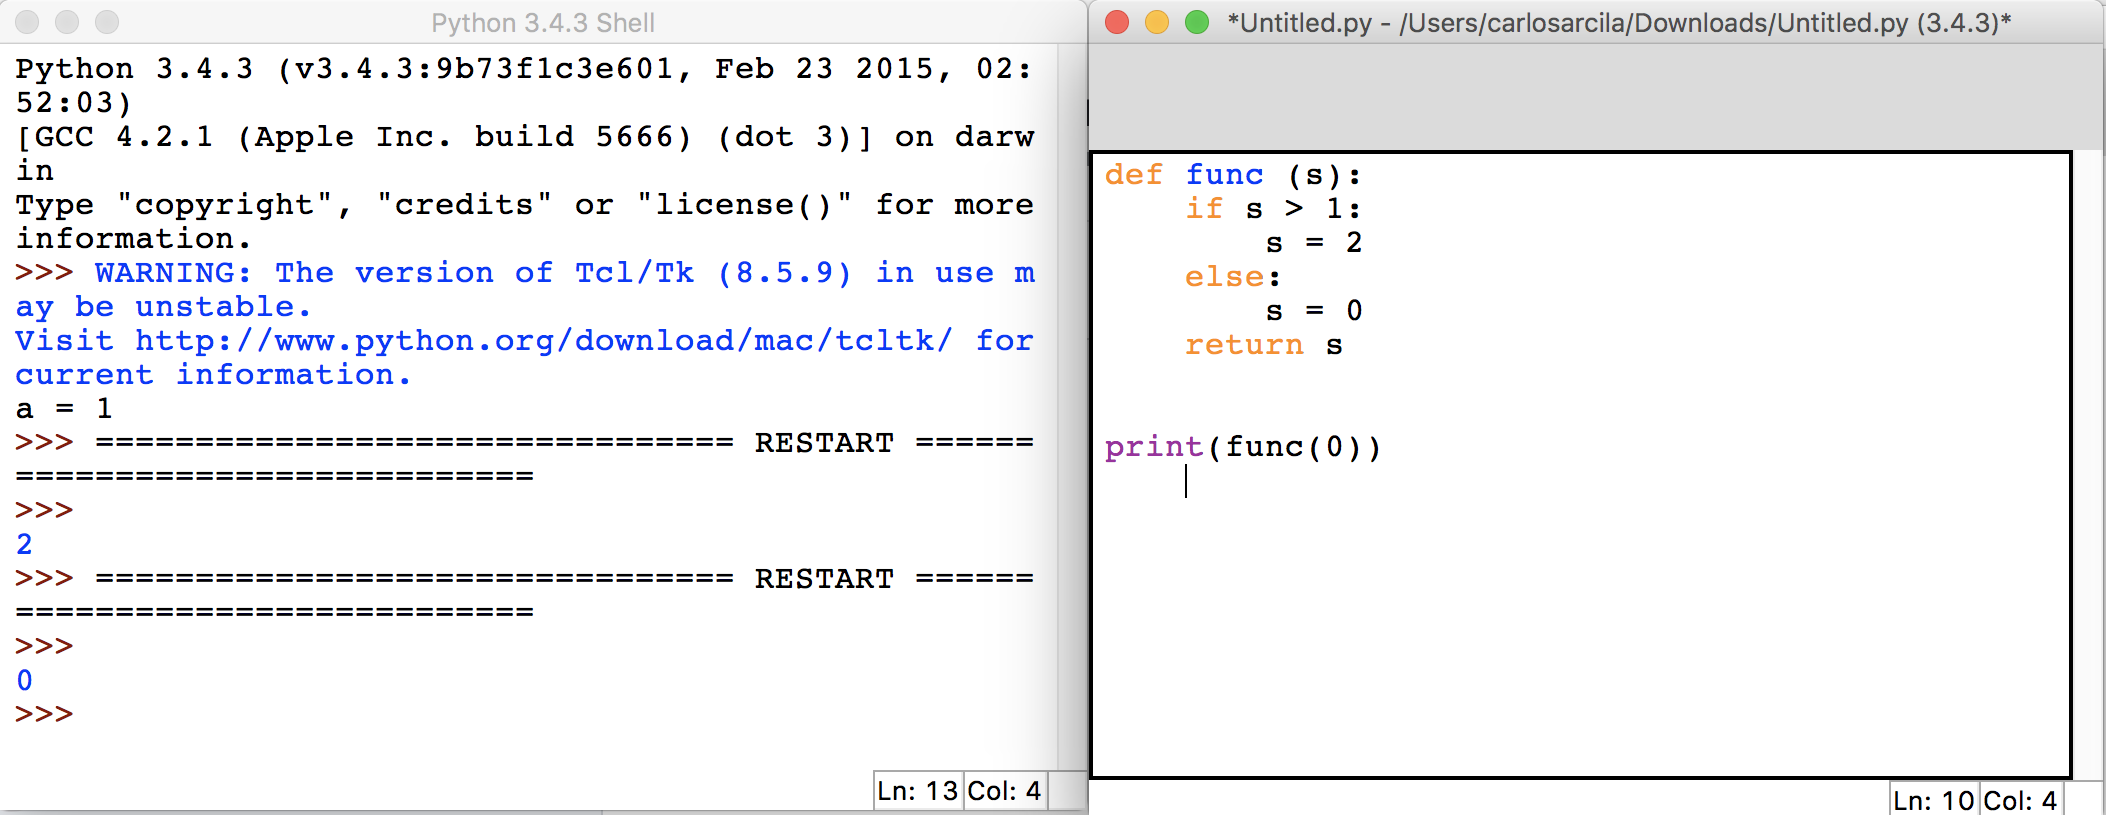
\includegraphics[width=0.9\linewidth]{figures/ch3_python_idle}
\caption{Python shell (left) and file (right) in IDLE.}
\label{fig:python_idle}
\end{figure}

While there is nothing wrong with using IDLE, most people will
find it a bit too limited and not tailored towards the needs of
a data analyst. We will therefore introduce three alternatives:
Spyder, Jupyter, and PyCharm.

Many people who move from R to Python like \pkg{spyder}, as it
looks pretty much like R Studio. Even if it is a bit less powerful,
it includes the same basic elements: a section to write a script,
a console for issuing ad-hoc commands (and reading output), and
a graphical overview of objects in the environment, here called
the variable inspector (Figure~\ref{fig:python_spyder}). 

\begin{figure}
\centering
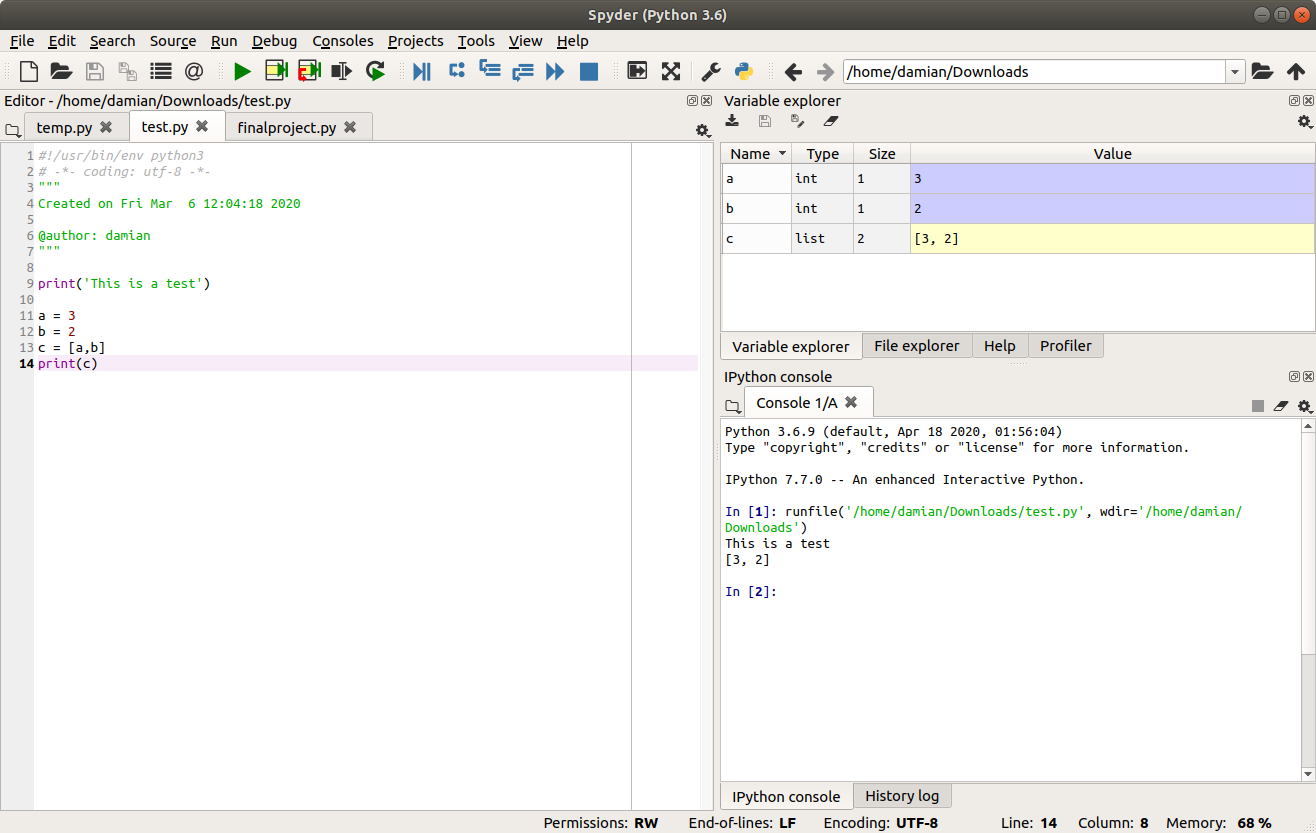
\includegraphics[width=0.9\linewidth]{figures/ch3-spyder}
\caption{A bit of an R feeling in Python: \pkg{spyder}}
\label{fig:python_spyder}
\end{figure}

Another popular way to write and run Python code in the realm of data
analysis are so-called \pkg{jupyter} notebooks. These notebooks, which
are also included in the IDE JupyterLab, are run as a web application
that allowsyou to create documents that contain live code and text
(and also equations and visualizations).  One of the nicest things of
the Jupyter Notebook is that the code is inserted in fields that you
can run one by one, getting its respective output, which added to the
designed narrative text will make your script more clean and
reproducible. You can also add formatted text blocks to explain to the
reader what you are doing. In \refsec{practices}, we will address
notebooks again as a good practice for a computational scientist.


Finally, we introduce \pkg{PyCharm}, an IDE that provides an even more
graphical and integrated interface to deal with Python than for
instance \pkg{spyder}. It is especially popular among programmers, and
many features may feel overwhelming if you are just about to start,
but it is an excellent choice, especially if you work on bigger projects.
Developed by JetBrains, PyCharm has a free and
open source \emph{Community} version that you can download and install
on your local computer from its
webpage\footnote{https://www.jetbrains.com/pycharm/download/} with
options for Windows, MacOS and Linux. Once installed you can connect
the software to any of the already installed versions of Python or
even easily create \emph{virtual environments} to work on your
projects. These virtual environments are isolated Python environments
that will let you have a specific configuration and dependencies to
work with in a project. For example, you may create one with an older
version of Python, including specific releases of libraries.  You can
equally achieve this with the pip command from your system terminal:
|pip install virtualenv|.
 
But PyCharm will help you to manage it with a graphical and friendly
interface. The same happens with installing packages: using the
\emph{Project} sub-menu from the \emph{Preferences} menu, you can
install, update and delete any package related to any version of
Python or virtual environment. In fact, easily dealing with Python
versions and libraries is one of the main reasons why we recommend to
new \emph{pythoners} to use PyCharm. But there are even more
advantages.

Just like RStudio, PyCharm is an integrated interface that shows us
different adjustable windows with a unique frame that we create for
every project we open. Every time you create a project you have to
name it, save it to a specific location (a folder where all your files
will be stored) and choose an interpreter (a Python version or
environment used by default in the project). Once created, you can
begin to work on it with three main windows or sub-frames
(Figure~\ref{fig:pycharm}). The upper-left window contains the project
structure and files. You can easily create or import folders and files
and then navigate through them in this area. For example, by clicking
on the right button of your mouse (or by going to File \textgreater
New) you can create a new Python file (i.e. my\_first\_script.py) and
organize your scripts by folders. In the upper-right window you will
be able to visualize and modify the editable files contained in a
project. All the open files will be in this window and you can access
to any of them by clicking on its name situated in the upper tabs. In
the low window you will find the output space as well as the Python
and system consoles. This separation is very useful since you can work
on your .py script (also with colour, indentation and error detection
facilities), run it (from the \emph{Run} Menu) and produce the
expected output in a separate window within the same frame.

\begin{figure}
\centering
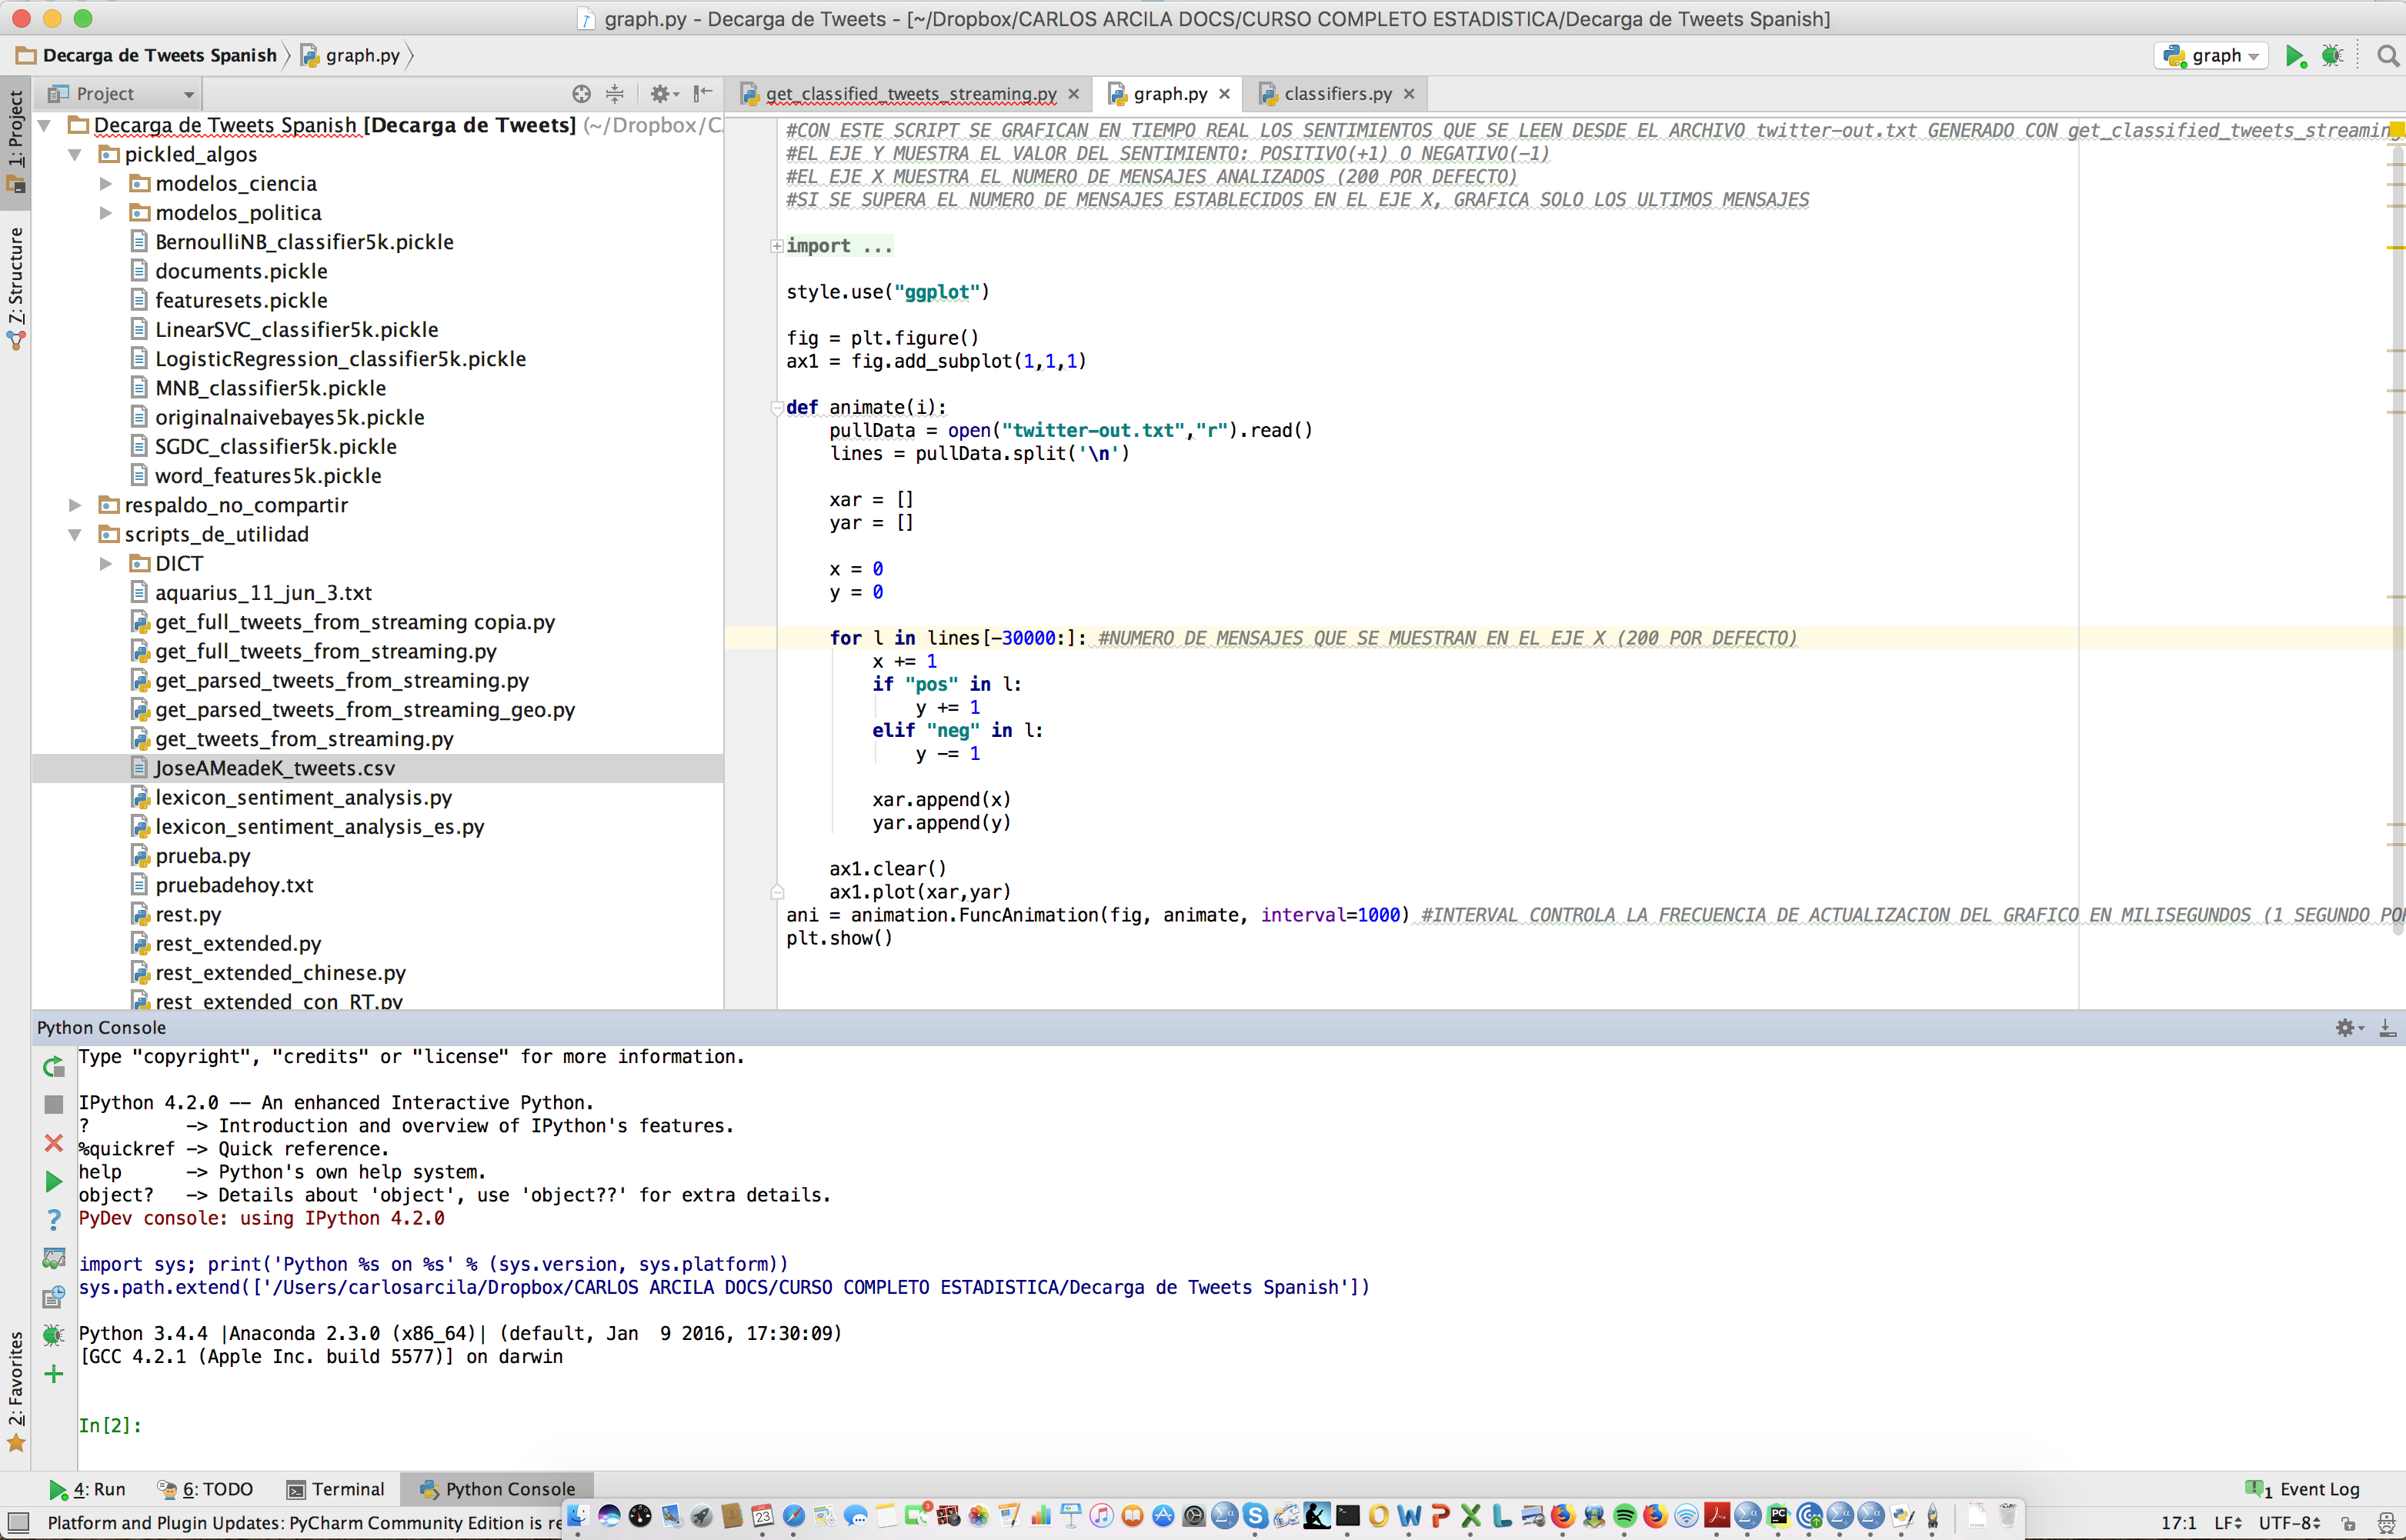
\includegraphics[width=0.9\linewidth]{figures/ch3_pycharm}
\caption{PyCharm environment.}
\label{fig:pycharm}
\end{figure}


It is important to notice that you do not have to install Python
\textit{and} Spyder \textit{and} Jupyter \textit{and} PyCharm \textit{and} Anaconda,
though it is typical that many computational scientist have different
IDEs in their computers. You can choose which of them are most
appropriate for your work -- and which one you feel most comfortable with.
